\documentclass[norsk,11pt,a4paper]{report}
\usepackage[margin=2.5cm,tmargin=2.5cm,bmargin=2.5cm,lmargin=2cm,rmargin=2cm,footskip=.2in]{geometry}
\title{REAL111-1 24H - Fysikk\\Labøving 1 - Elektrisitet}
\author{Eivind N. Sognnes, Elias Fossdal, Casper Eide Özdemir-Børretzen, Elias Olai Skog}
\date{}

% % % % % % % % % % % % % % % % % % % % % % % % % % % % % % % % % % % % % % % % 

\usepackage{babel}               % Support for other languages than english
\usepackage{nicefrac}            % Nice looking fractals
\usepackage{mhchem}              % Chemistry symbols
\usepackage{graphicx}            % Images
\usepackage{listings}            % Code
\usepackage{ulem}                % Double underline
\usepackage{amssymb}             % ...
\usepackage{pdfpages}            % Insert pdf pages
\usepackage{enumitem}            % Lists
\usepackage{titlesec}            % ...
\usepackage[T1]{fontenc}         % ...
\usepackage[utf8]{inputenc}      % ...
%\usepackage[fleqn]{amsmath}      % ...
\usepackage[makeroom]{cancel}    % ...
\usepackage{pgfplots}            % Graphs
\pgfplotsset{width=10cm,compat=1.9}
\setlength{\parindent}{0pt}
\titlespacing*{\subsection}{0cm}{1.5cm}{0.5cm}
\lstset{
aboveskip=0cm,
belowskip=0cm,
showstringspaces=false,
columns=flexible,
basicstyle={\scriptsize\ttfamily},
breaklines=true,
breakatwhitespace=true,
tabsize=4,
inputencoding = utf8,  % Input encoding
extendedchars = true,  % Extended ASCII
literate      =        % Support additional characters
{á}{{\'a}}1  {é}{{\'e}}1  {í}{{\'i}}1 {ó}{{\'o}}1  {ú}{{\'u}}1
{Á}{{\'A}}1  {É}{{\'E}}1  {Í}{{\'I}}1 {Ó}{{\'O}}1  {Ú}{{\'U}}1
{à}{{\`a}}1  {è}{{\`e}}1  {ì}{{\`i}}1 {ò}{{\`o}}1  {ù}{{\`u}}1
{À}{{\`A}}1  {È}{{\`E}}1  {Ì}{{\`I}}1 {Ò}{{\`O}}1  {Ù}{{\`U}}1
{ä}{{\"a}}1  {ë}{{\"e}}1  {ï}{{\"i}}1 {ö}{{\"o}}1  {ü}{{\"u}}1
{Ä}{{\"A}}1  {Ë}{{\"E}}1  {Ï}{{\"I}}1 {Ö}{{\"O}}1  {Ü}{{\"U}}1
{â}{{\^a}}1  {ê}{{\^e}}1  {î}{{\^i}}1 {ô}{{\^o}}1  {û}{{\^u}}1
{Â}{{\^A}}1  {Ê}{{\^E}}1  {Î}{{\^I}}1 {Ô}{{\^O}}1  {Û}{{\^U}}1
{œ}{{\oe}}1  {Œ}{{\OE}}1  {æ}{{\ae}}1 {Æ}{{\AE}}1  {ß}{{\ss}}1
{ẞ}{{\SS}}1  {ç}{{\c{c}}}1 {Ç}{{\c{C}}}1 {ø}{{\o}}1  {Ø}{{\O}}1
{å}{{\aa}}1  {Å}{{\AA}}1  {ã}{{\~a}}1  {õ}{{\~o}}1 {Ã}{{\~A}}1
{Õ}{{\~O}}1  {ñ}{{\~n}}1  {Ñ}{{\~N}}1  {¿}{{?`}}1  {¡}{{!`}}1
{„}{\quotedblbase}1 {“}{\textquotedblleft}1 {–}{$-$}1
{°}{{\textdegree}}1 {º}{{\textordmasculine}}1 {ª}{{\textordfeminine}}1
{£}{{\pounds}}1  {©}{{\copyright}}1  {®}{{\textregistered}}1
{«}{{\guillemotleft}}1  {»}{{\guillemotright}}1  {Ð}{{\DH}}1  {ð}{{\dh}}1
{Ý}{{\'Y}}1    {ý}{{\'y}}1    {Þ}{{\TH}}1    {þ}{{\th}}1    {Ă}{{\u{A}}}1
{ă}{{\u{a}}}1  {Ą}{{\k{A}}}1  {ą}{{\k{a}}}1  {Ć}{{\'C}}1    {ć}{{\'c}}1
{Č}{{\v{C}}}1  {č}{{\v{c}}}1  {Ď}{{\v{D}}}1  {ď}{{\v{d}}}1  {Đ}{{\DJ}}1
{đ}{{\dj}}1    {Ė}{{\.{E}}}1  {ė}{{\.{e}}}1  {Ę}{{\k{E}}}1  {ę}{{\k{e}}}1
{Ě}{{\v{E}}}1  {ě}{{\v{e}}}1  {Ğ}{{\u{G}}}1  {ğ}{{\u{g}}}1  {Ĩ}{{\~I}}1
{ĩ}{{\~\i}}1   {Į}{{\k{I}}}1  {į}{{\k{i}}}1  {İ}{{\.{I}}}1  {ı}{{\i}}1
{Ĺ}{{\'L}}1    {ĺ}{{\'l}}1    {Ľ}{{\v{L}}}1  {ľ}{{\v{l}}}1  {Ł}{{\L{}}}1
{ł}{{\l{}}}1   {Ń}{{\'N}}1    {ń}{{\'n}}1    {Ň}{{\v{N}}}1  {ň}{{\v{n}}}1
{Ő}{{\H{O}}}1  {ő}{{\H{o}}}1  {Ŕ}{{\'{R}}}1  {ŕ}{{\'{r}}}1  {Ř}{{\v{R}}}1
{ř}{{\v{r}}}1  {Ś}{{\'S}}1    {ś}{{\'s}}1    {Ş}{{\c{S}}}1  {ş}{{\c{s}}}1
{Š}{{\v{S}}}1  {š}{{\v{s}}}1  {Ť}{{\v{T}}}1  {ť}{{\v{t}}}1  {Ũ}{{\~U}}1
{ũ}{{\~u}}1    {Ū}{{\={U}}}1  {ū}{{\={u}}}1  {Ů}{{\r{U}}}1  {ů}{{\r{u}}}1
{Ű}{{\H{U}}}1  {ű}{{\H{u}}}1  {Ų}{{\k{U}}}1  {ų}{{\k{u}}}1  {Ź}{{\'Z}}1
{ź}{{\'z}}1    {Ż}{{\.Z}}1    {ż}{{\.z}}1    {Ž}{{\v{Z}}}1  {ž}{{\v{z}}}1
}

% % % % % % % % % % % % % % % % % % % % % % % % % % % % % % % % % % % % % % % % 

\newcommand{\oppgave}[2]{\item[#1:] #2}
\newcommand{\oppgaveDelStart}{\begin{enumerate}[leftmargin=*,itemsep=0.25cm,labelsep=1.5em,label=\alph*)]}
\newcommand{\oppgaveDelSlutt}{\end{enumerate}}
\newcommand{\oppgaveDel}[1]{\item[#1)]}

% % % % % % % % % % % % % % % % % % % % % % % % % % % % % % % % % % % % % % % % 

\begin{document}
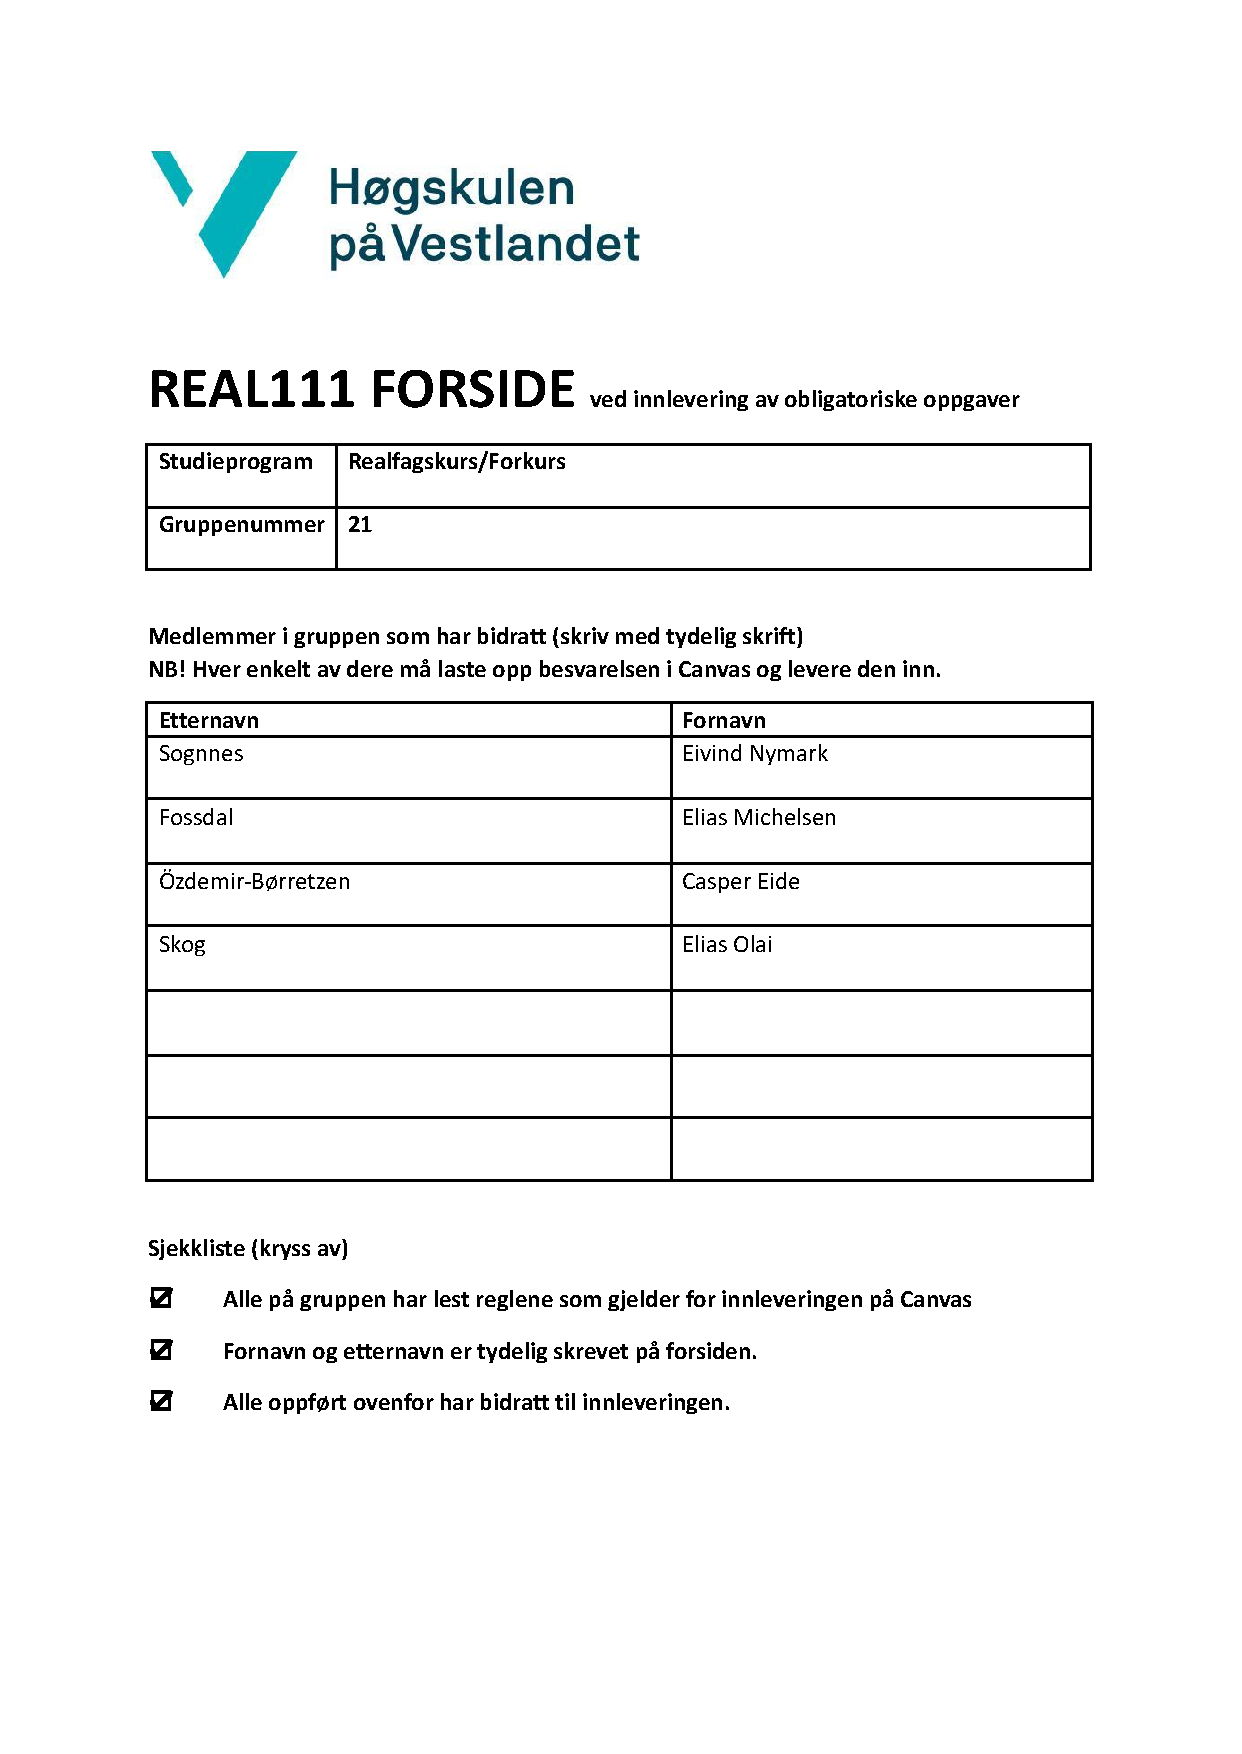
\includepdf[pages={1}]{real111-forside.pdf}

% % % % % % % % % % % % % % % % % % % % % % % % % % % % % % % % % % % % % % % % 

\section*{Laboratorierapport 1 av 2: Elektrisitet}
Gruppe: Eivind N. Sognnes, Elias Fossdal, Casper Eide Özdemir-Børretzen, Elias Olai Skog

\subsection*{Innledning}
I denne laboratorieøvelsen skal vi undersøke om formlene og teorien fra læreboken om motstander i serie- og parallell-koblinger er korrekt.\\[0.2cm]

Motstand i serie $\rightarrow \boxed{R_s = R_1 + R_2}$\\[0.2cm]

Motstand i parallell $\rightarrow \boxed{\frac{1}{R_p} = \frac{1}{R_1} + \frac{1}{R_2}}$\\[0.2cm]

Vi skal ta i bruk et $4,5V$ batteri, to lyspærer, elektrisk motor med tilhørende propell, kabler med krokodilleklemmer og et multimeter i øvelsen.

\subsection*{Resultater}
Videre følger måleresultater, samt beregninger som er gjort under øvelsen.\\
\begin{enumerate}[itemsep=1cm]

\oppgave{1}{Få lyspæren til å lyse}\\\\
I første del av øvelsen målte vi spenningen på batteriet uten belastning, dette kalles elektromagnetisk spenning eller ems forkortet. Måling av emsen ga resultatet $4,37\ V$. Videre koblet vi opp en krets med en enkel lyspære og tok måling av spenningen over lyspæren, ved å koble multimeteret parallelt med pæren. I tillegg målte vi strømmen gjennom kretsen, ved å koble multimeteret i serie.
\oppgaveDelStart{}
\oppgaveDel{a} Måling av spenningsfall: $4,37\ V \rightarrow 3,10\ V$
\oppgaveDel{b} Måling av strømmen i kretsen: $0,22\ A$
\oppgaveDel{c} Beregning av motstand: $R = \frac{U}{I} = \frac{3,10\ V}{0,22\ A} = 14,1\ \Omega$
\oppgaveDel{d} Her kan det være flere feilkilder. Dårlig kontakt på et eller flere punkter i kretsen kan være en mulig feilkilde. Eksempelvis ved at lyspæren ikke er skrudd helt inn, at koblingspunktene ved lyspæren er løse eller ved at krokodilleklemmene er dårlig festet og har kordeller som er brukket eller henger løst. En annen mulig feilkilde er unøyaktig måleinstrument. Under øvelsen brukte vi et multimeter fra Biltema (art.nr. 15-133) med feilmargin oppgitt til $\pm\ 0,5\ \%$ ved innstilling på $20V\ DC$ måling og $\pm\ 2\ \%$ ved måling av strøm i $10\ A$ innstillingen.
\oppgaveDelSlutt{}

\newpage

\oppgave{2}{Seriekobling av lyspærer}\\\\
Her har vi utvidet kretsen ved å koble inn enda en lyspære i serie med den forrige.
\oppgaveDelStart
\oppgaveDel{a} Lysstyrken har blitt svakere etter at den andre pæren ble koblet inn. Begge pærene har lik lysstyrke.
\oppgaveDel{b} Spenningen over pærene er $1,77V$ og $1,70V$. Over begge pærene samlet er spenningen $3,48V$.
\oppgaveDel{c} Måling av strømmen i kretsen: $0,18\ A$
\oppgaveDel{d} Teoretisk er resistansen til de to pærene i serie gitt ved:\\[0.2cm]
$\boxed{R_s = R_1 + R_2}$\\[0.2cm]
Med resistansen beregnet fra tidligere gir det:\\[0.2cm]
$R_s = 14,1\ \Omega + 14,1\ \Omega = 28,2\ \Omega$\\[0.2cm]
Resistansen beregnet fra målingene gjort på de to pærene i serie gir:\\[0.2cm]
$R_1 = \frac{1,77\ V}{0,18\ A} = 9,833\ \Omega$\\[0.2cm]
$R_2 = \frac{1,70\ V}{0,18\ A} = 9,444\ \Omega$\\[0.2cm]
$R_s = R_1 + R_2 = 9,833\ \Omega + 9,444\ \Omega = 19,278\ \Omega$\\[0.2cm]
Resistansen beregnet fra målingen gjort over begge pærene samlet:\\[0.2cm]
$R_s = \frac{3,48\ V}{0,18\ A} = 19,333\ \Omega$\\[0.2cm]
Resistansen målt i seriekretsen stemmer \uline{ikke} med resistansen fra tidligere måling. Dette er fordi resistansen i glødepærer vil variere med temperaturen. Temperaturen vil variere med strømmen og spenningen over pæren. I en seriekobling er som vist i pkt. b spenningen over pærene mindre enn i oppg. 1.
\oppgaveDelSlutt

\oppgave{3}{Parallellkobling av lyspærer}\\\\
I denne delen av øvelsen har vi koblet om pærene som var seriekoblet til å være parallellkoblet.
\oppgaveDelStart
\oppgaveDel{a} Spenningen målt over lyspærene er $2.87V$ og $2,40V$. Spenningen målt over begge pærene samlet er $2,40V$. Dette stemmer \uline{ikke} overens med hva vi hadde forventet fra teorien. Utifra det vi har lært om spenningsfall i parallellkobling burde alle tre målingene ha gitt samme resultat. Ulikt resultat på målingene skyldes nok mest sannsynlig samme feilkilder som nevnt i oppg. 1d.
\oppgaveDel{b} Spenningen målt mellom polene er $3,60V$. Dette er \uline{ikke} lik spenningen over de to pærene. Avvik kan skyldes dårlig kontakt på et eller flere punkter i kretsen eller motstand i ledningene. Vi erfarte store variasjoner ved små bevegelser i ledningene. Noe som understøtter teorien om dårlig kontakt og stor motstand i ledningene.
\oppgaveDelSlutt

\newpage
\oppgave{4}{Elektromotorisk spenning og indre resistans}\\
I neste steg av øvelsen har vi fjernet den ene parallellkoblede lyspæren og erstattet den med en motor med propell.
\oppgaveDelStart
\oppgaveDel{a} Da pæren ble utbyttet med motoren ble lysstyrken i den gjenværende pæren \uline{svakere}.
\oppgaveDel{b} Da vi fjernet propellen fra motoren ble lysstyrken \uline{sterkere}.
\oppgaveDel{c} Når vi bremset motoren med hånden ble lysstyrken \uline{litt svakere}.
\oppgaveDel{d} At lysstyrken faller i pkt. a når motoren med propell kobles til indikerer at motoren i startøyeblikket trekker mer strøm enn lyspæren den erstattet, på grunn av lav indre motstand og lav elektromotorisk spenning. Siden dette er en parallellkobling, er spenningen over motoren og lyspæren den samme, men den økte totale strømmen gjennom kretsen fører til et større spenningsfall over batteriets indre resistans. Dette gjør at spenningen som faktisk når lyspæren blir lavere, og den lyser svakere.\\

Når propellen fjernes reduseres den mekaniske belastningen på motoren. Motoren roterer da raskere og utvikler høyere elektromotorisk spenning (motspenning), noe som fører til at motoren trekker mindre strøm. Dette reduserer spenningsfallet over batteriets indre resistans, og spenningen over lyspæren øker --- dermed lyser den sterkere.\\

Når motoren bremses med hånden (pkt. c), økes den mekaniske belastningen, rotasjonshastigheten synker, og den elektromotoriske spenningen blir mindre. Dette gjør at motoren trekker mer strøm, og spenningsfallet over batteriets indre resistans øker igjen. Lyspæren får da lavere spenning og lyser svakere.
\oppgaveDelSlutt

\newpage
\oppgave{Ekstra}{Plotte $I$-$U$-karakteristikk}
\oppgaveDelStart
\oppgaveDel{a}\ \\
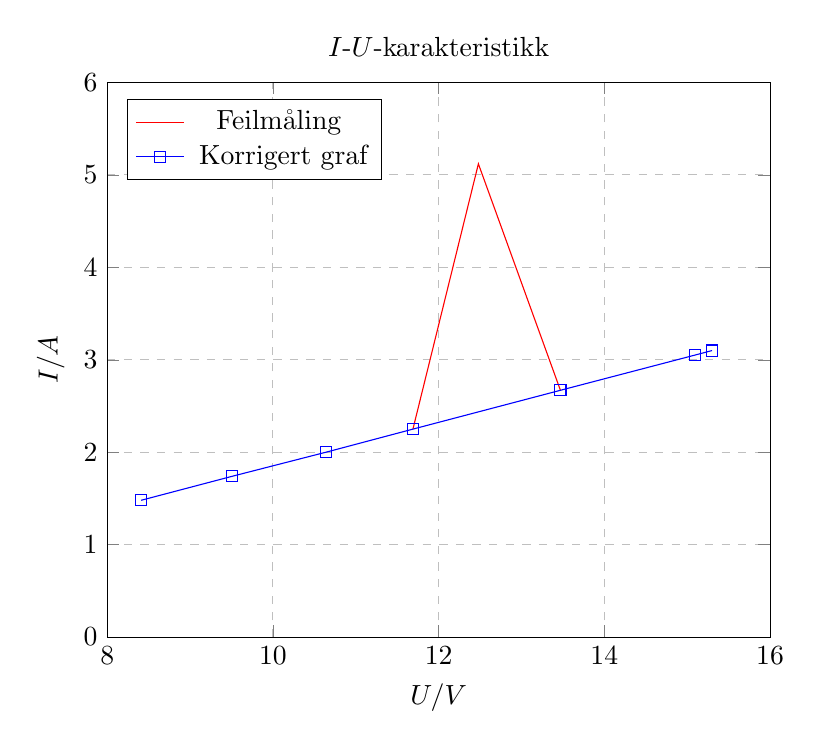
\begin{tikzpicture}
\begin{axis}[
title={$I$-$U$-karakteristikk},
xlabel={$U/V$},
ylabel={$I/A$},
xmin=8, xmax=16,
ymin=0, ymax=6,
xtick={8,10,12,14,16},
ytick={0,1,2,3,4,5,6},
legend pos=north west,
ymajorgrids=true,
xmajorgrids=true,
grid style=dashed,
]
\addlegendentry{Feilmåling}
\addplot[
color=red,
]
coordinates {
(11.69, 2.25)
(12.48, 5.12)
(13.47, 2.67)
};
\addplot[
color=blue,
mark=square,
]
coordinates {
( 8.41, 1.48)
( 9.51, 1.74)
(10.64, 2.00)
(11.69, 2.25)
(13.47, 2.67)
(15.09, 3.05)
(15.30, 3.10)
};
\addlegendentry{\ Korrigert graf}
\end{axis}
\end{tikzpicture}

\oppgaveDel{b}\ \\
\begin{tabular}{| l | l | l |}
\hline
$U/V$ & $I/A$  & $R/\Omega$\\
\hline
 8,41 &  1,48  & 5,68 \\
 9,51 &  1,74  & 5,47 \\
10,64 &  2,0   & 5,32 \\
11,69 &  2,25  & 5,20 \\
12,48 &  5,12* & \sout{2,44} \\
13,47 &  2,67  & 5,04 \\
15,09 &  3,05  & 4,95 \\
15,30 &  3,10  & 4,94 \\
\hline
\end{tabular}\\[0.2cm]
* Feilmåling

\oppgaveDel{c} Komponenten har varierende resistans og er \uline{ikke} ohmsk.

%\oppgaveDel{d} Den absolutte feilen er: $A = x \pm \delta A$

\oppgaveDelSlutt

\end{enumerate}

\subsection*{Konklusjon}
Øvelsen ble utført, men ga til tider annet resultat enn forventet. Dette skyldes gjerne feil på utstyr eller andre feil under måling av verdier. For videre utdyping av mulige feilkilder se resultat i oppgave 1d. Oppsummert så skyldes trolig de største avvikene dårlig kontakt i overgangen mellom ledning og krokodilleklemme. På tross av dette viser resultatet at teorien for både serie og parallellkobling stemmer overens med praksis og målingene observert i denne øvelsen. Det største avviket som strider mot teorien opplevde vi i oppgave 3a og b. Basert på tilgjengelig teori forventet vi her at alle målingene skulle ha vært tilnærmet like siden det er snakk om parallellkobling og spenningsmålinger over de to lyspærene og batteriet. Siden det var store variasjoner på målt resultat ved små bevegelser i ledninger og kontakter konkluderer vi derfor med at avviket skyldes utstyret og at teorien derfor stemmer.

% % % % % % % % % % % % % % % % % % % % % % % % % % % % % % % % % % % % % % % % 

\end{document}
